\documentclass[11pt]{standalone}
\usepackage{amssymb}
\usepackage{amsmath}
\usepackage[no-math]{fontspec}
\usepackage{unicode-math}
\setmainfont{Libertinus Sans}
\setsansfont{Libertinus Sans}
\setmathfont{Libertinus Math}
\usepackage{pgf,xcolor}
\usepackage{tikz}
\usetikzlibrary{arrows.meta, backgrounds}
\usepackage{pgfplots}
\pgfplotsset{compat=newest}
\usepackage{pifont}

\definecolor{my_darkgray}{HTML}{484949}
\definecolor{my_lightgray}{HTML}{F3F4F4}
\definecolor{my_darkblue}{HTML}{005A94}
\definecolor{my_lightblue}{HTML}{CCDEE9}
\definecolor{my_yellow}{HTML}{FFEC7F}
\definecolor{my_red}{HTML}{E60000}
\definecolor{my_orange}{HTML}{E87846}

% Gitter im Abstand 0.1 m und Achsen, in jedem Panel gleich
\newcommand{\koordinatensystem}{%
    \draw[gitter, step=0.1] (-0.2,-0.2) grid (0.9,0.5);
    \draw[achse] (-0.2,0) -- (0.9,0)
        node[anchor=north east, font=\small, text=my_darkgray] {$x$};
    \draw[achse] (0,-0.2) -- (0,0.5)
        node[anchor=north east, font=\small, text=my_darkgray] {$y$};
}

\begin{document}
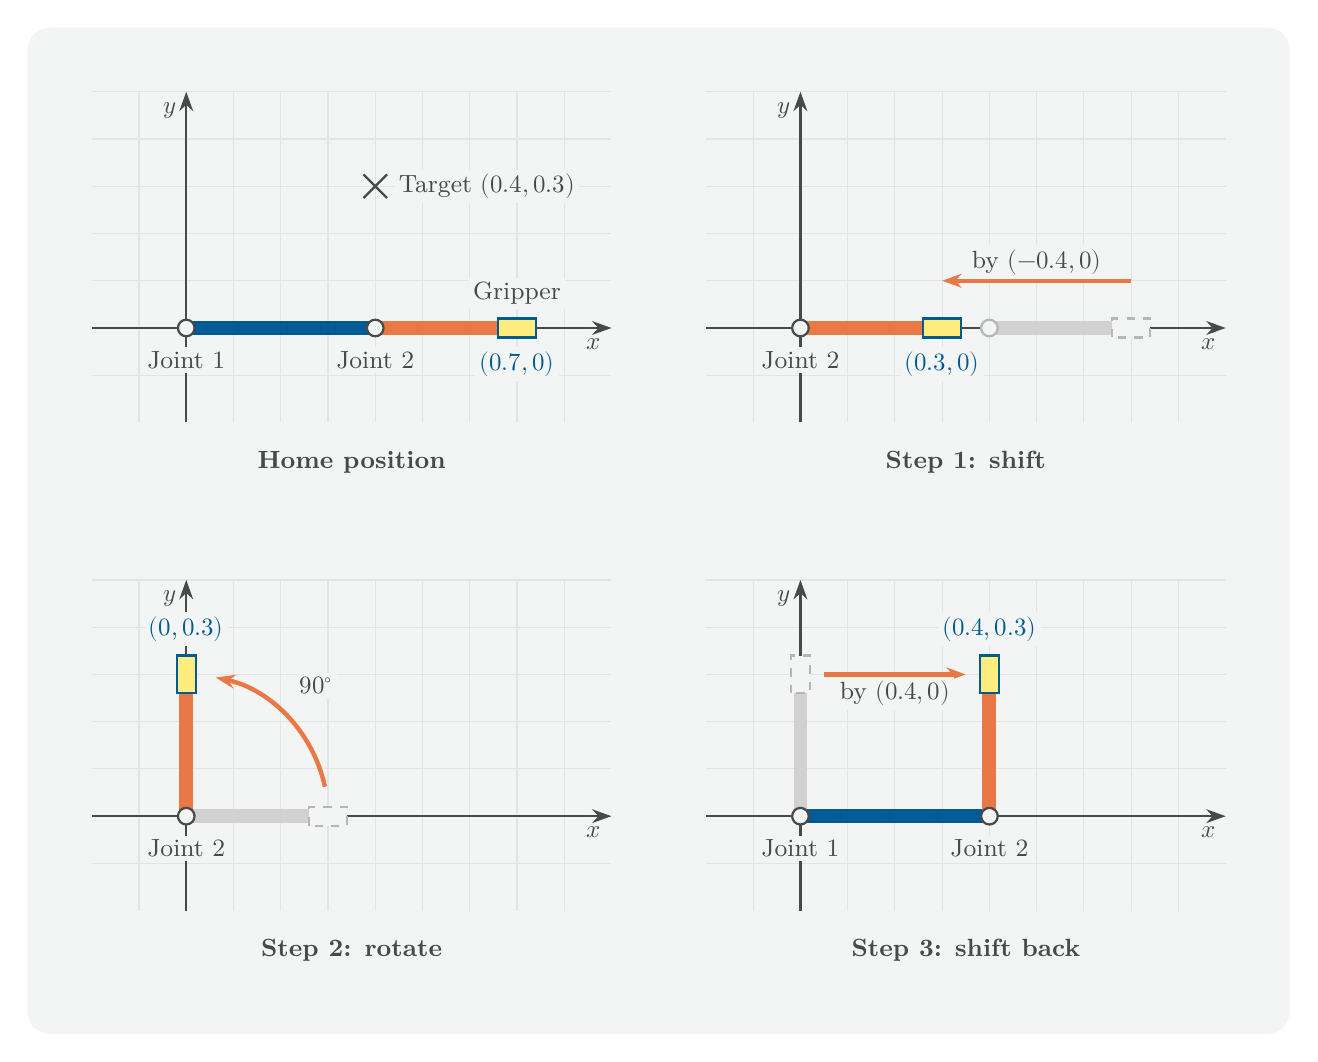
\begin{tikzpicture}[
    show background rectangle,
    background rectangle/.style={fill=my_lightgray, rounded corners=8pt},
    inner frame sep=0.8cm,
    % Maßstab: 1 m = 6 cm, alle Koordinaten in m
    x=6cm, y=6cm,
    gitter/.style={draw=my_darkgray!15, line width=0.4pt},
    achse/.style={draw=my_darkgray, thick, -{Stealth[length=7pt, width=5pt]}},
    bewegung/.style={draw=my_orange, ultra thick, -{Stealth[length=7pt, width=5pt]}},
    arm1/.style={draw=my_darkblue, line width=5pt, line cap=round},
    arm2/.style={draw=my_orange, line width=5pt, line cap=round},
    schatten/.style={draw=my_darkgray!25, line width=5pt, line cap=round},
    gelenk/.style={fill=my_lightgray, draw=my_darkgray, thick},
    gelenkschatten/.style={fill=my_lightgray, draw=my_darkgray!40, thick},
    bauteil/.style={fill=my_yellow, draw=my_darkblue, thick},
    bauteilschatten/.style={fill=my_lightgray, draw=my_darkgray!40, thick, dashed},
    beschriftung/.style={font=\small, text=my_darkgray, fill=my_lightgray, inner sep=1.5pt},
    koordinate/.style={font=\small, text=my_darkblue, fill=my_lightgray, inner sep=1.5pt},
    titel/.style={font=\small\bfseries, text=my_darkgray, anchor=north}
]

    % Farbig: Stellung nach dem Schritt, grau: Stellung vor dem Schritt.
    % In den Schritten 1 und 2 rechnen wir nur mit Arm 2 und dem Bauteil.

    % ===== Panel 1: Grundstellung =====
    \begin{scope}
        \koordinatensystem

        % Ziel des Greifers als Kreuz
        \draw[draw=my_darkgray, thick] (0.4,0.3) +(-0.025,-0.025) -- +(0.025,0.025)
            +(-0.025,0.025) -- +(0.025,-0.025);
        \node[beschriftung, anchor=west] at (0.44,0.3) {Target $(0.4, 0.3)$};

        % Gestreckter Arm
        \draw[arm1] (0,0) -- (0.4,0);
        \draw[arm2] (0.4,0) -- (0.7,0);
        \draw[gelenk] (0,0) circle (3pt);
        \draw[gelenk] (0.4,0) circle (3pt);
        \draw[bauteil] (0.66,-0.02) rectangle (0.74,0.02);

        % Beschriftungen
        \node[beschriftung, anchor=north] at (0,-0.04) {Joint 1};
        \node[beschriftung, anchor=north] at (0.4,-0.04) {Joint 2};
        \node[beschriftung, anchor=south] at (0.7,0.04) {Gripper};
        \node[koordinate, anchor=north] at (0.7,-0.04) {$(0.7, 0)$};

        \node[titel] at (0.35,-0.24) {Home position};
    \end{scope}

    % ===== Panel 2: Schritt 1, Gelenk 2 in den Ursprung verschieben =====
    \begin{scope}[xshift=7.8cm]
        \koordinatensystem

        % Vorher: Arm 2 in der Ausgangslage
        \draw[schatten] (0.4,0) -- (0.7,0);
        \draw[gelenkschatten] (0.4,0) circle (3pt);
        \draw[bauteilschatten] (0.66,-0.02) rectangle (0.74,0.02);

        % Nachher: Gelenk 2 liegt im Ursprung
        \draw[arm2] (0,0) -- (0.3,0);
        \draw[gelenk] (0,0) circle (3pt);
        \draw[bauteil] (0.26,-0.02) rectangle (0.34,0.02);

        % Weg des Greifers
        \draw[bewegung] (0.7,0.1) -- (0.3,0.1)
            node[midway, beschriftung, anchor=south] {by $(-0.4, 0)$};

        % Beschriftungen
        \node[beschriftung, anchor=north] at (0,-0.04) {Joint 2};
        \node[koordinate, anchor=north] at (0.3,-0.04) {$(0.3, 0)$};

        \node[titel] at (0.35,-0.24) {Step 1: shift};
    \end{scope}

    % ===== Panel 3: Schritt 2, um den Ursprung drehen =====
    \begin{scope}[yshift=-6.2cm]
        \koordinatensystem

        % Vorher: Arm 2 nach Schritt 1
        \draw[schatten] (0,0) -- (0.3,0);
        \draw[bauteilschatten] (0.26,-0.02) rectangle (0.34,0.02);

        % Nachher: um 90 Grad um den Ursprung gedreht
        \draw[arm2] (0,0) -- (0,0.3);
        \draw[gelenk] (0,0) circle (3pt);
        \draw[bauteil] (-0.02,0.26) rectangle (0.02,0.34);

        % Weg des Greifers auf dem Kreis um den Ursprung
        \draw[bewegung] (12:0.3) arc[start angle=12, end angle=78, radius=0.3];
        \node[beschriftung] at (45:0.39) {$90^\circ$};

        % Beschriftungen
        \node[beschriftung, anchor=north] at (0,-0.04) {Joint 2};
        \node[koordinate, anchor=south] at (0,0.36) {$(0, 0.3)$};

        \node[titel] at (0.35,-0.24) {Step 2: rotate};
    \end{scope}

    % ===== Panel 4: Schritt 3, Gelenk 2 an seinen Platz zurückverschieben =====
    \begin{scope}[xshift=7.8cm, yshift=-6.2cm]
        \koordinatensystem

        % Vorher: Arm 2 nach Schritt 2
        \draw[schatten] (0,0) -- (0,0.3);
        \draw[bauteilschatten] (-0.02,0.26) rectangle (0.02,0.34);

        % Nachher: Arm 1 ist stehen geblieben, Arm 2 sitzt wieder an Gelenk 2
        \draw[arm1] (0,0) -- (0.4,0);
        \draw[arm2] (0.4,0) -- (0.4,0.3);
        \draw[gelenk] (0,0) circle (3pt);
        \draw[gelenk] (0.4,0) circle (3pt);
        \draw[bauteil] (0.38,0.26) rectangle (0.42,0.34);

        % Weg des Greifers
        \draw[bewegung] (0.05,0.3) -- (0.35,0.3)
            node[midway, beschriftung, anchor=north] {by $(0.4, 0)$};

        % Beschriftungen
        \node[beschriftung, anchor=north] at (0,-0.04) {Joint 1};
        \node[beschriftung, anchor=north] at (0.4,-0.04) {Joint 2};
        \node[koordinate, anchor=south] at (0.4,0.36) {$(0.4, 0.3)$};

        \node[titel] at (0.35,-0.24) {Step 3: shift back};
    \end{scope}

\end{tikzpicture}
\end{document}
